\chapter{Microfabrication}

Our next step was to fabricate a device capable of performing FMR on our samples while applying a DC-Bias in order to modulate the damping \cite{IRGENDWAS WAS DC-BIAS macht}. This required creating an isolation layer between the DC lines and the FMR lines. This chapter will explain the methods attempted to create this isolation layer via cross-linking of a photoresist, as well as the actual process of fabrication for the device.

\section{Optimizing the cross-linking process}
To create the device's isolation layer, photoresist cross-linking was identified as the optimal method. We tested several cross-linking techniques to determine the most effective approach for device fabrication, which are detailed in the following.
\subsection{e-Beam lithography}
We first attempted cross-linking via our e-Beam lithography machine (EBL). For this, the $\textit{AR-N 7520.17 new}$ photoresist was spin-coated onto a silicon sample at 4000 rpm with an acceleration of 1000 rpm/s. The sample was then soft-baked at 85C$^\circ$ for one minute and placed into the EBL. The electron beam was set to 20kV and the aperture set to 20µm, with a beam current of 112pA and a padding of 6mm/s.

To verify that our concept works, we exposed a small square on the sample with the side length of 100µm with a dose of 10000 µC/cm$^2$, which was done by exposing the same area to 100 µC/cm$^2$ a hundred times. For reference, the dose recommended by the manufacturer is 30 µC/cm$^2$ \cite{Allresist_ARN7520}. After the exposure, the sample was developed with the $\textit{AR300-47}$ developer for around 50 seconds, and was submerged into deionized water for 30 seconds.

Following the development, a series of stress tests were done which included applying a pressurized stream of acetone onto the sample, submerging the sample into a acetone bath at 60C$^\circ$ for 10 minutes. Subsequently, the sample was submerged in the $AZ351B$ developer for two minutes. Finally, the sample was put into an ultrasonic acetone bath at the highest setting (9/9) we have available at the lab for one minute. This last step was done to really test the durability of the cross-linking. In the actual sample, ultrasonic bath is only needed for the process of removing gold from the sample, called liftoff, where we only use the lowest setting (1/9).

The sample seemed to withstand the acetone stream well, but changes in the color were visible after the acetone bath and the developer. The ultrasonic acetone bath washed only the failed attempts of exposure away, indicating that the cross-linking was successful and durable. The exposure took around three hours, however, which is long considering the size of the exposed area. Since the area we wanted to expose on the real sample was significantly larger, we needed to find a way to reduce the time taken for the exposure.

In order to find the minimal dose necessary to accomplish this task, we tried different doses on the same sample, which is shown in figure \ref{fig:dose-exposure}. The exposure was done in layers of exposures of 100 µC/cm$^2$.
\begin{figure}
    \centering
    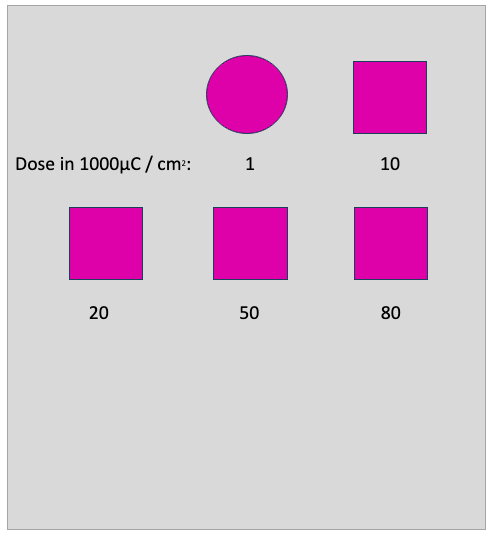
\includegraphics[width=0.6\linewidth]{chapters/Photos/Microfabrication/E-line Dose.png}
    \caption{Sample illustration of the exposure done with the EBL. The first exposed area is a circle to be able to differentiate between up and down. The exposure was done in layers of 100 µC/cm$^2$.}
    \label{fig:dose-exposure}
\end{figure}

After the exposure, the sample was developed with the $\textit{AR300-47}$ developer for around two minutes, followed by a 30 second submersion in deionized water. The sample then underwent the same stress tests as before.
Some color changes were visible in the areas exposed with one to 20 layers of 100 µC/cm$^2$ after the acetone pressure stream, and the acetone bath seemed to make the area with 50 layers appear brighter. The $\textit{AZ351B}$ developer seemed to have no effect on the sample, but the ultrasonic fully removed the area exposed only once, as well as corroded the areas with 10 and 20 layers at the edges slightly.
In the end, we concluded that a dose of 20000 µC/cm$^2$ (20 layers) was the sweet spot between time taken and durability. The corroded edges were deemed acceptable for the actual sample, as they would not impair the performance of the device.

With this dose, the exposure should have taken around 15 hours on a real sample. When trying this on a real sample, however, the EBL shut down after seven hours. The reason remains unknown, but the most probable cause is thought to be the large aperture and beam current. Since the design we wanted to expose was fairly large, we opted for an aperture of 60$\mu m$, which resulted in a beam current of 1113pA. This was significantly larger than other exposures done in the past on the machine by other researchers. The long duration of this exposure could have also resulted in an overheating of the cathode. 

Given this, another method was investigated where three corners of a sample with the $\textit{AR-N 7520.17 new}$ photoresist were looked at with the EBL for 1, 5 and 10 minutes, respectively. After this, the sample underwent a stress test using an acetone bath and the $\textit{AR300-47}$ developer. The corner that was stared at for only a minute washed away immediately in the acetone bath. The corner that was exposed for five minutes could be seen even after the bath, even though significant damage was visible through the microscope, which is shown in figure \ref{fig:5min}.
\begin{figure}[htbp] % [htbp] for flexible placement
    \centering % Center the entire figure
    \begin{subfigure}[c]{0.48\textwidth} 
        \subcaption{} % Place (a) above the image
        \centering
        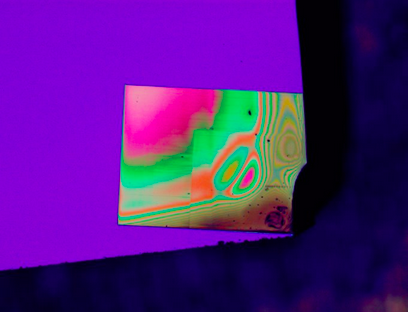
\includegraphics[width=\linewidth,height = 6cm]{chapters/Photos/Microfabrication/5min_before.png}
        \label{fig:5min_before}
    \end{subfigure}
    \hfill % Flexible horizontal space
    \begin{subfigure}[c]{0.48\textwidth} 
        \subcaption{} % Place (b) above the image
        \centering
        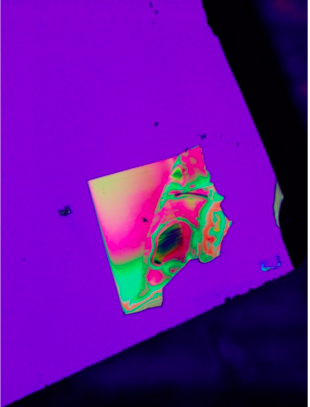
\includegraphics[width=\linewidth, height = 6cm]{chapters/Photos/Microfabrication/5min_after.png} 
        \label{fig:5min_after}
    \end{subfigure}
    \hfill % Flexible horizontal space
    \caption{Image of the corner of the sample that was exposed for five minutes. The damage is clearly visible, but the corner is still intact. Image (a) shows the sample before the acetone bath, while image (b) shows it after the bath.}
    \label{fig:5min} % Main label for the entire figure
\end{figure}
The corner that was exposed for 10 minutes was still intact after the acetone bath and the developer, but variances in color were visible, pointing to a THICKNESS VARIANCE? The pictures taken under the microscope are shown in figure \ref{fig:10min}. The damage was not as severe as in the five-minute corner, but it was still significant, which is why this method was not pursued further. 
\begin{figure}
    % I want three pictures in one row
    \centering
    \begin{subfigure}[c]{0.32\textwidth} 
        \subcaption{} % Place (a) above the image
        \centering
        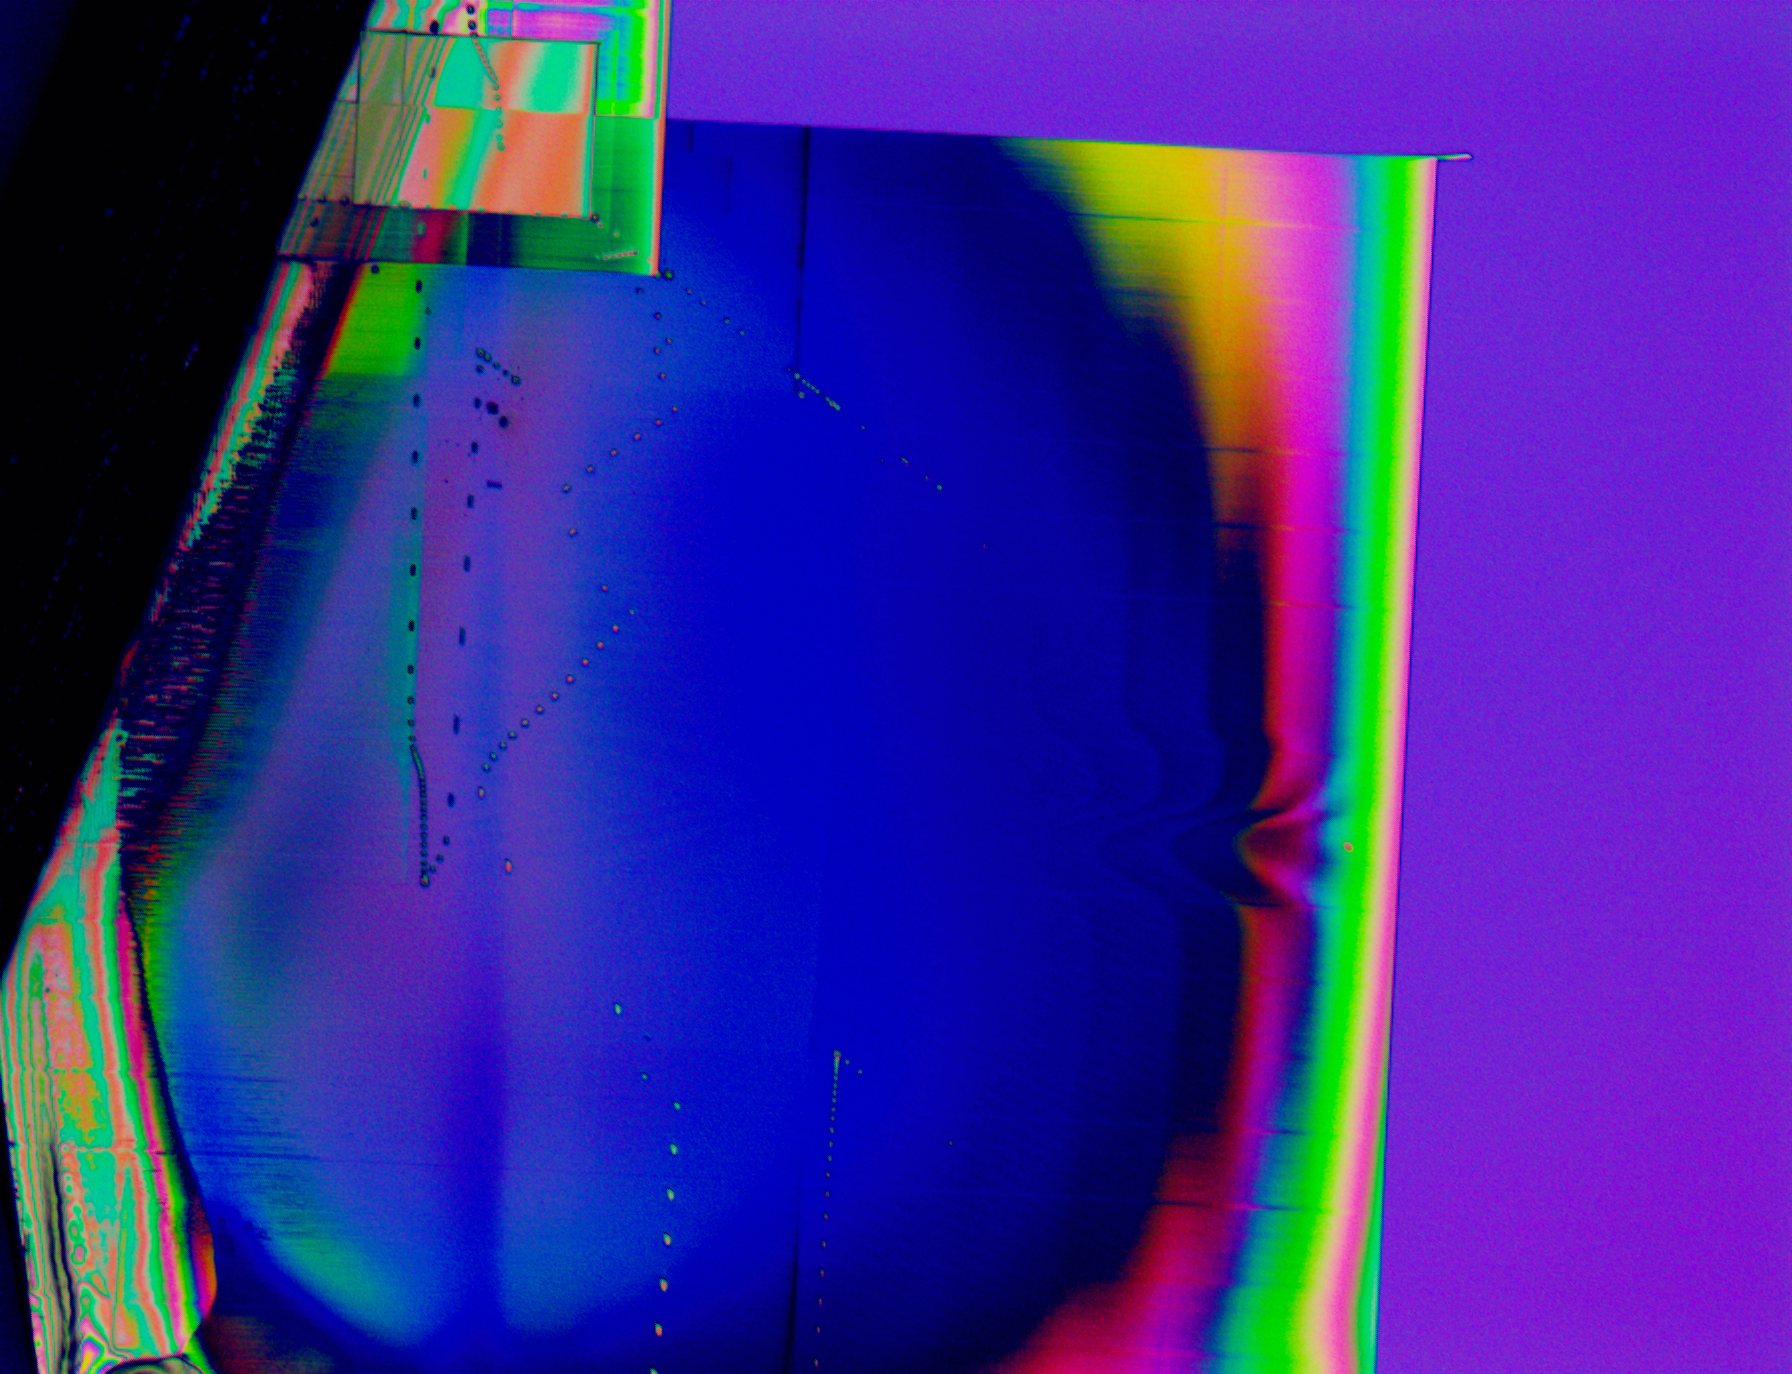
\includegraphics[width=\linewidth]{chapters/Photos/Microfabrication/10min_looking_ebeam.png}
        \label{fig:10min_before}
    \end{subfigure}
    \hfill % Flexible horizontal space
    \begin{subfigure}[c]{0.32\textwidth} 
        \subcaption{} % Place (b) above the image
        \centering
        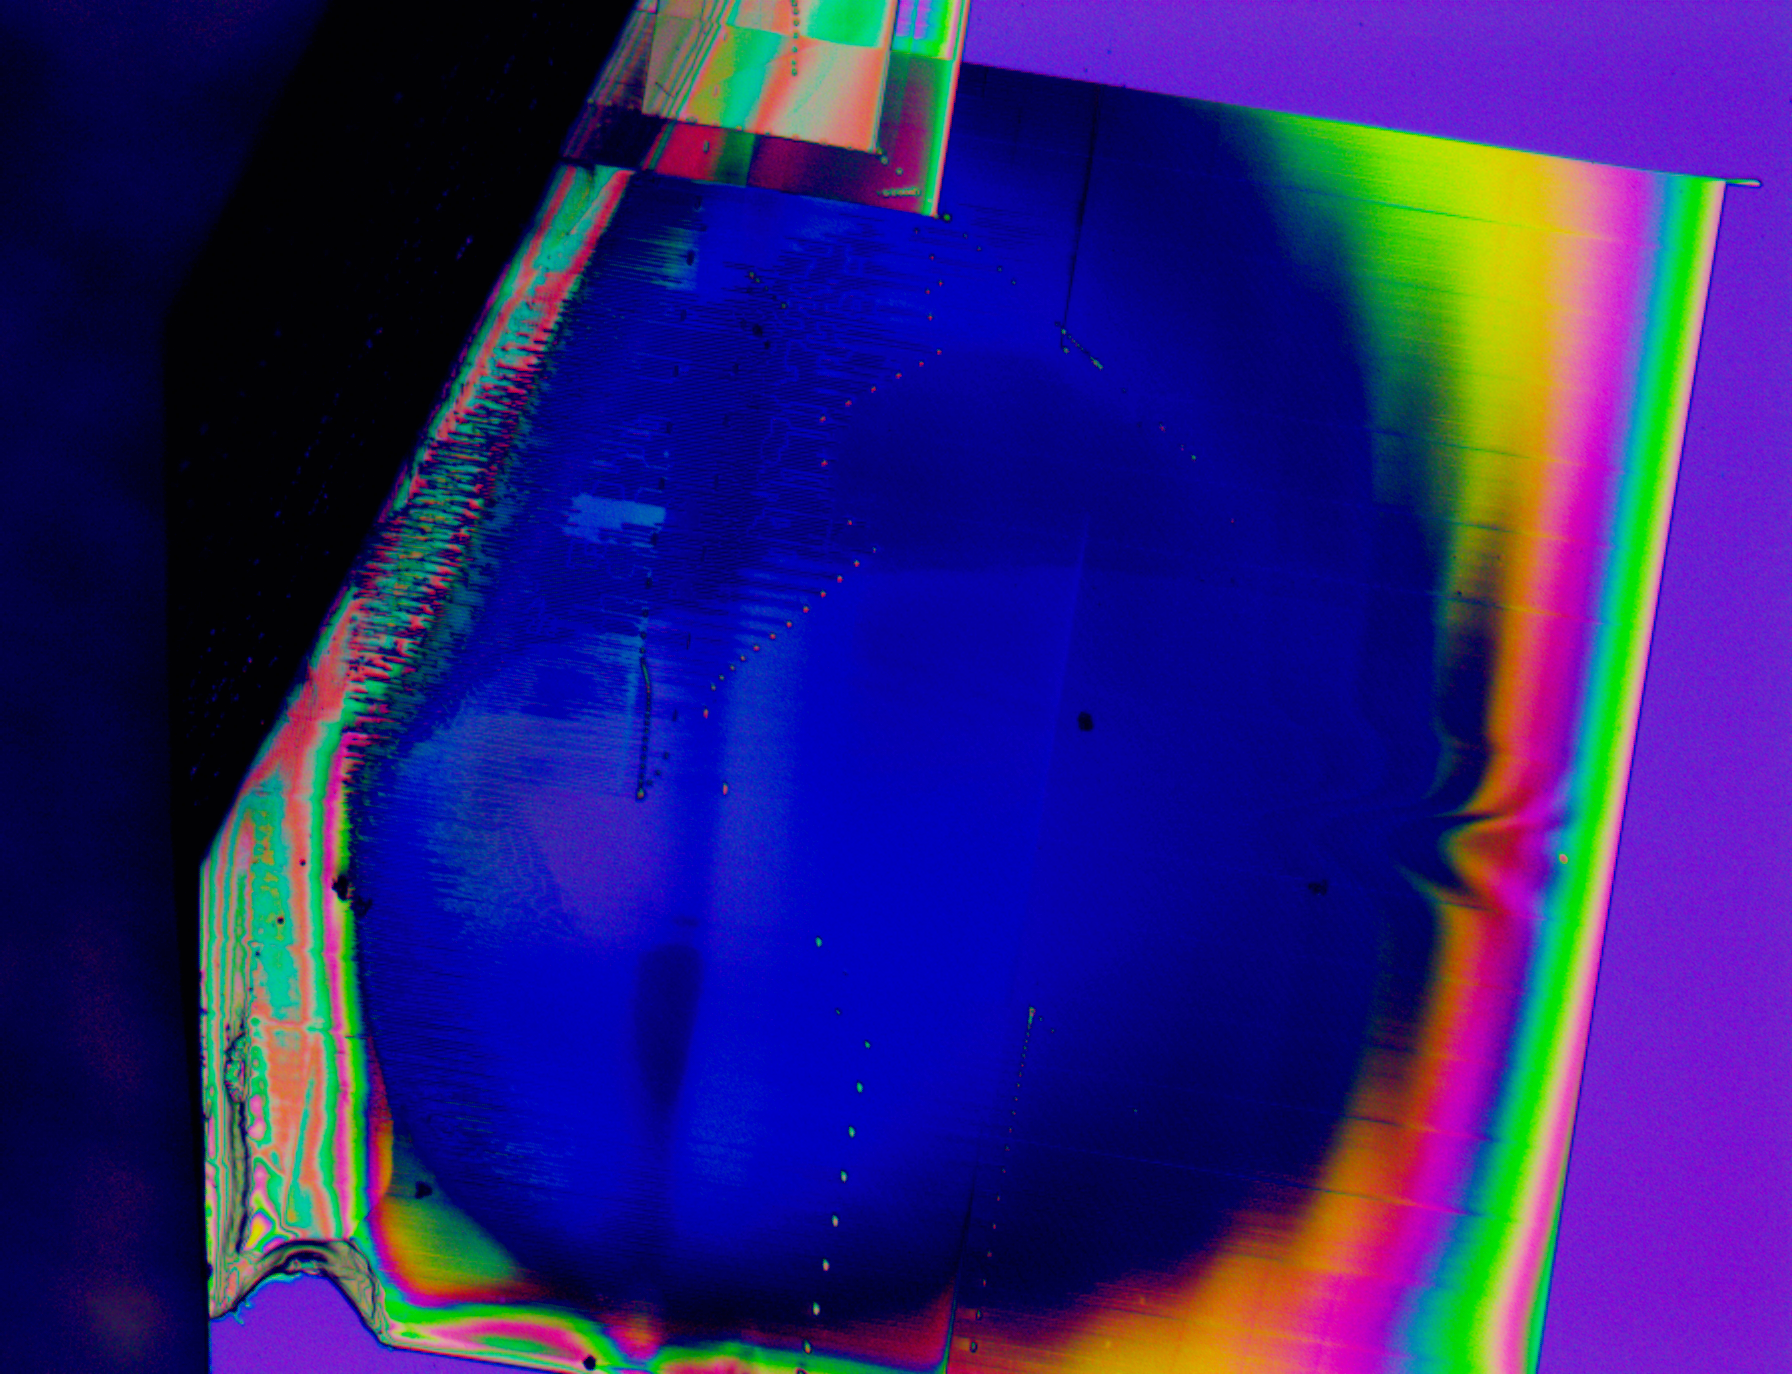
\includegraphics[width=\linewidth]{chapters/Photos/Microfabrication/10min_looking_ebeam_after_bath.png} 
        \label{fig:10min_after_bath}
    \end{subfigure}
    \hfill % Flexible horizontal space
    \begin{subfigure}[c]{0.32\textwidth} 
        \subcaption{} % Place (c) above the image
        \centering
        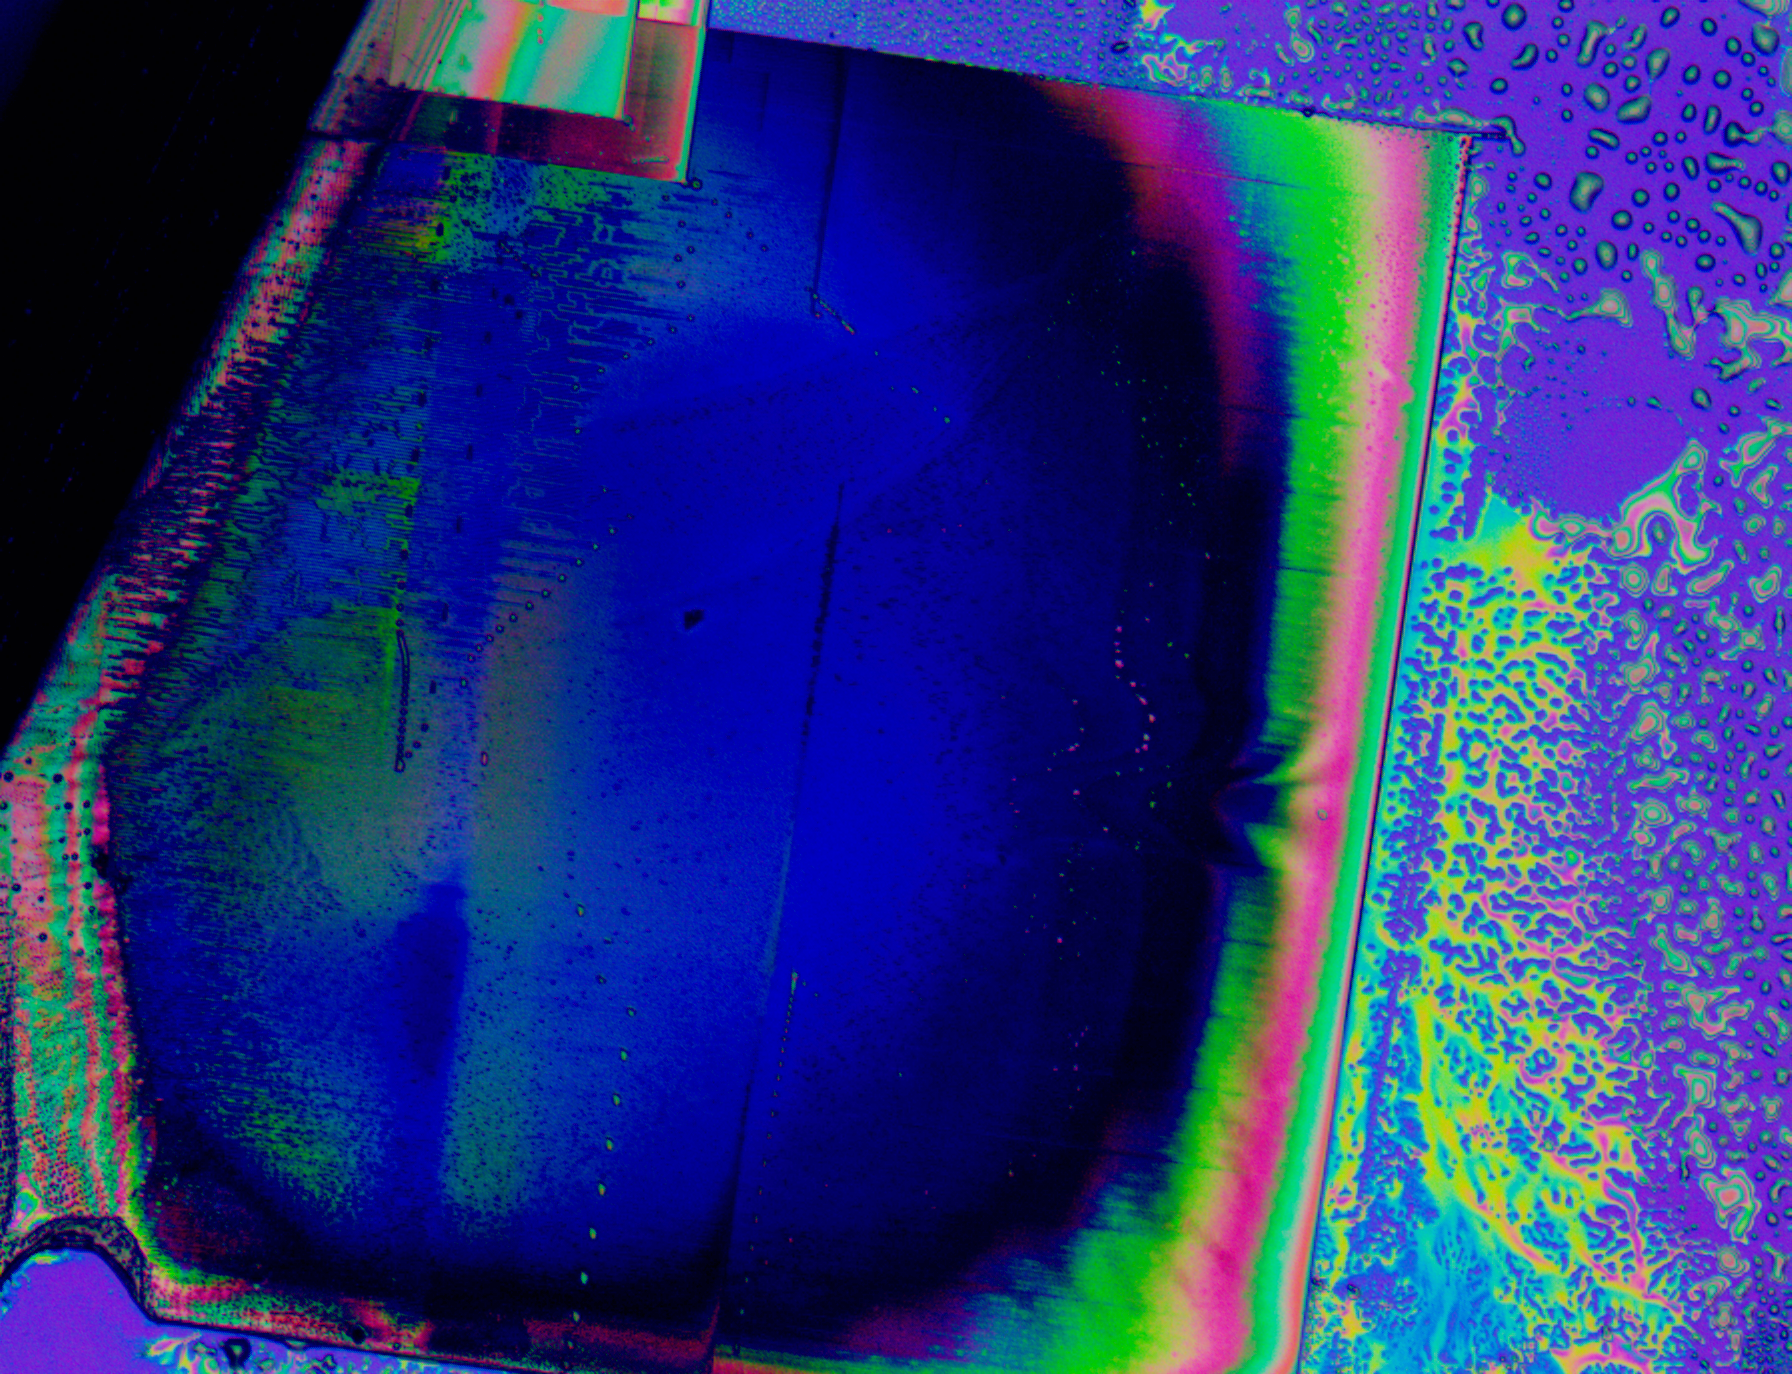
\includegraphics[width=\linewidth]{chapters/Photos/Microfabrication/10min_looking_ebeam_after_bath_and_dev.png} 
        \label{fig:10min_after_dev} 
    \end{subfigure}
    \hfill % Flexible horizontal space
    \caption{Image of the corner of the sample that was exposed for 10 minutes. Image (a) shows the sample before the acetone bath, image (b) shows it after the bath and image (c) shows it after the developer. There are certain spots visible that change its color in (c), possibly pointing to a variance in thickness.}
    \label{fig:10min} % Main label for the entire figure
\end{figure}

\subsection{MLA} 
After the several attempts with the EBL, our focus shifted to the MLA. We used the same $\textit{AR-N 7520.17 new}$ photresist, spincoated it onto a silicon sample and exposed different spots with different doses, similar to the procedure with the EBL machine. We have tested doses from 800-2300 µC/cm$^2$ to pinpoint the sweet spot between time taken and the dose needed. 
After the exposure, the sample underwent the same stress test procedure as the samples exposed with the EBL to investigate its chemical tolerance against the steps that the actual isolation layer will need to withstand. The ultra sonic bath was omitted, however. 
After the acetone stream, some spots were visible on some dose. The acetone bath seemed to have some effect, especially on the lower doses, but the sample was still intact for the higher doses.

This method showed great durability and seemed to be able to withstand the stress test, even at a dose of 1000 µC/cm$^2$. However, there were multiple stripes visible on the sample at all doses, which pointed to a high variance in thickness. To test this, we used an atomic force microscope (AFM) to investigate the thickness of the photoresist, which is shown in figure \ref{AFM_1}.

ENTER AFM EXPLANATION 

After the AFM measurement, we tried dividing the exposure into multiple steps and rotating the sample between the steps to even out the stripes. This, however, showed no significant improvement. This method was therefore deemed unfit for the isolation layer, as the variance in thickness would lead to an uneven surface for the CPW. (MAYBE WRITE DIFFERENTLY). Another researcher at the chair (Sam Fülop CHECK NAME), however, found out after the conclusion of my work that that the issue with the stripes can be resolved by applying a significantly higher dose of around 20000(CHECK) µC/cm$^2$, which is the main way cross-linking is now done at the chair.
\subsection{Microscope}
We also investigated whether exposing the photoresist with a microscope would be a viable option. For this, we used the $\textit{MA-N 1407}$ photoresist which we spin-coated onto a slilicon sample at ENTER RPM SETTING, followed by a softbake at 100C$^\circ$ for 5 minutes. The sample was then exposed with a microscope for 10min at ENTER MAGNIFICATION. After the exposure, the sample was developed with the ENTER DEVELOPER developer and put into deionized water for 30 seconds. Subsequently, an acetone stream was applied onto the sample. Unfortunately, the sample did not withstand the process and the photoresist washed away completely. This method was therefore deemed unfit for the isolation layer.

\subsection{Overbaking}
Finally, we investigated whether overbaking the photoresist, as in doing the pre-baking process significantly longer than recommended, would lead to a durable isolation layer.
For this, we have spincoated samples with both the $\textit{AR-N 7520.17 new}$ and the $\textit{MA-N 1407}$ photoresist onto silicon samples at their respective recommended RPM settings which are detailed in the sections above. The samples were then put onto a hotplate at 100C$^\circ$ for 20 minutes to overbake them.

Both samples then underwent stress tests which included pressurized acetone streams, submersion in their respective developer, and acetone baths. The overbaked sample with the $\textit{AR-N 7520.17 new}$ photoresist was damaged AFTER WHAT?
The sample with the $\textit{MA-N 1407}$ photoresist, however, withstood the stress test and and stayed in tact after an acetone bath of 10 minutes AT WHAT TEMP?, although there were some holes visible in the isolation layer, which are shown in figure \ref{holes}.

\section{Fabrication of samples}

    - lithography of gold-plates
    - cross-linking through MLA
    - lithography of CPW -> etching -> gold dampfen
    - Insert soldering and bonding of sample to insert 